\pdfoutput=1
\documentclass[pra,twocolumn,showpacs,amsmath,amssymb]{revtex4-2}

\usepackage{graphicx}%Include figure files
\usepackage{dcolumn}%Align table columns on decimal point
\usepackage{bm}% bold math
\usepackage[section]{placeins} %force no floats before section
\usepackage{float}
\usepackage{amsmath}

%\setlength{\parskip}{1em}

%\nofiles

\begin{document}

\title{Phys460 Project 1: Radioactive Decay in a Two Nuclei System}


\author{Christopher McGlinn}
\affiliation{Department of Physics and Astronomy, University
of Delaware, Newark, DE 19716-2570, USA}

\begin{abstract}
Radioactive decay is a natural phenomenon that occurs when a nucleus spontaneously decays into another and emits radiation. In this scenario, the first nuclei decays into the second one, and from there decays further. This decay is reflected through a series of equations as will be described in this article. This article will discuss how the two nuclei act over time while comparing the analytical solution to a numerical solution using the Euler method.
\end{abstract}

\pacs{23}


\maketitle

\section{Introduction} \label{sec:intro}

Radioactive decay was first discovered by Henri Becquerel in 1896 while studying phosphorescent materials. Since that time, the field has been extensively explored.

\par Radioactivity occurs when the an element decays into another element and emits energy in the form of particles. These particles can take the form of an alpha or beta particle, or it can take the form of a neutrino. The system loses energy when that particle is emitted from the system. Often times a nucleus will decay into a different kind of nucleus, which in turn decays further.

\par In the situation described in this article, one nuclei decays into another one, which then decays further. Consider the following two equations:

\begin{align}
\frac{dN_A}{dt} &= -\frac{N_A}{\tau_A}\\
\frac{dN_B}{dt} &= \frac{N_A}{\tau_A} - \frac{N_B}{\tau_B}
\end{align}

\par Here we can see a clear decay in the number of A particles. We also see that the decay of the B nuclei is dependent upon the quantity of both nuclei in the system. As such, nuclei A decays into nuclei B at a rate dependent upon the the time constant \(\tau_{A}\). As for \(\tau_{B}\), I will explore the differences between three situations \(\tau_A > \tau_B\), \(\tau_A < \tau_B\), and \(\tau_A = \tau_B\) given the initial conditions \(N_A(0) = 200\), \(N_B(0) = 10\), and \(\tau_A = 1\). I will show that the numeric approximation can be used to accurately reflect the decay of the system.


\section{Method} \label{sec:method}


To start off, we will normalize the given equations. For this, we will use a set of normalized variables and their differential forms:

\begin{align}
    t &= t_{o}\bar{t} & dt &= t_{o}d\bar{t} \notag \\
    N_{A} &= N_{A_{o}}\bar{N_{A}} & dN_{A} &= N_{A_{o}}d\bar{N_{A}} \notag \\
    N_{B} &= N_{B_{o}}\bar{N_{B}} & dN_{B} &= N_{B_{o}}d\bar{N_{B}} \notag
\end{align}

\par Starting off with Equation 1, it can further be simplified into:

\begin{equation}
\frac{d\bar{N}_A}{d\bar{t}} = -\frac{\bar{N}_A}{\tau_A}t_o
\end{equation}

\par Whereas Equation 2 can be simplified into:

\begin{align}
\frac{N_{B_o}}{t_o} \frac{d\bar{N}_B}{d\bar{t}} &= N_{A_o} \frac{\bar{N}_A}{\tau_A} - N_{B_o} \frac{\bar{N}_B}{\tau_B} \notag \\
\frac{d\bar{N}_B}{d\bar{t}} &= \frac{N_{A_o}}{N_{B_o}} \frac{\bar{N}_A}{\tau_A} t_o - \frac{\bar{N}_B}{\tau_B} t_o
\end{align}

From here we can further simplify Equation 3 and Equation 4 by setting the initial normalized vales equal to each other, $N_{A_o} = N_{B_o}$, and setting \(t_o = \tau_a\):

\begin{align}
\frac{d\bar{N}_A}{d\bar{t}} &= -\bar{N}_A\\
\frac{d\bar{N}_B}{d\bar{t}} &= \bar{N}_A - \frac{\bar{N}_B}{\tau_B}
\end{align}

Using the Euler method we come up with a numeric solution to the problem:
\begin{align}
N_{A_{i+1}} &= N_{A_i} - N_{A_i} \Delta t\\
N_{B_{i+1}} &= N_{B_i} + N_A \Delta t - \frac{N_B}{\tau_B} \Delta t
\end{align}

Since this method is an approximation, it is important to compare it to an analytical approach to see how accurate it is. For this we would need to solve the ordinary differential equations formed from equations 1:
\begin{align}
    \frac{dN_A}{N_A} = - \frac{dt}{\tau_A} \notag
\end{align}
Solving this gives us the equation:
\begin{align}
    N_{A}(t) &= N_{A_{o}}e^{-\frac{t}{\tau_{A}}}
\end{align}
As for equation 2, we can plug in equation 9 and solve for the complementary and particular solutions:
\begin{align}
\frac{dN_B}{dt} + &\frac{N_B}{\tau_B} = \frac{N_{A_o}}{\tau_A}e^{-\frac{t}{\tau_{A}}} \notag \\
N_{B}(t) = \frac{N_{A_{o}} \tau_B}{\tau_A-\tau_B}e^{-\frac{t}{\tau_{A}}} &+ (N_{B_{o}} - \frac{N_{A_{o}} \tau_B}{\tau_A-\tau_B})e^{-\frac{t}{\tau_{B}}}
\end{align}

This equation works well for the cases where $\tau_A \neq \tau_B$. However, in the case where they are equal we will need a third equation. This can be obtained by setting them equal to each other and then solving the differential equation. This results in the following equation:

\begin{align}
    N_B = N_{B_o}e^{-\frac{t}{\tau_A}} + \frac{N_{A_o}t}{\tau_A}e^{-\frac{t}{\tau_A}}
\end{align}

With these sets of equations we can plot the set of equations above to compare the numerical and analytical solutions. The results were calculated with \(\Delta t = 0.01\) and \(\tau_B = 0.5 , 1 , 1.5\).

\section{Results} \label{sec:results}

These are the results of evaluating the expressions for the scenarios \(\tau_A > \tau_B\), \(\tau_A < \tau_B\), and \(\tau_A = \tau_B\). First we will look at the decay of nuclei A in each of these scenarios:

\begin{figure}[H]
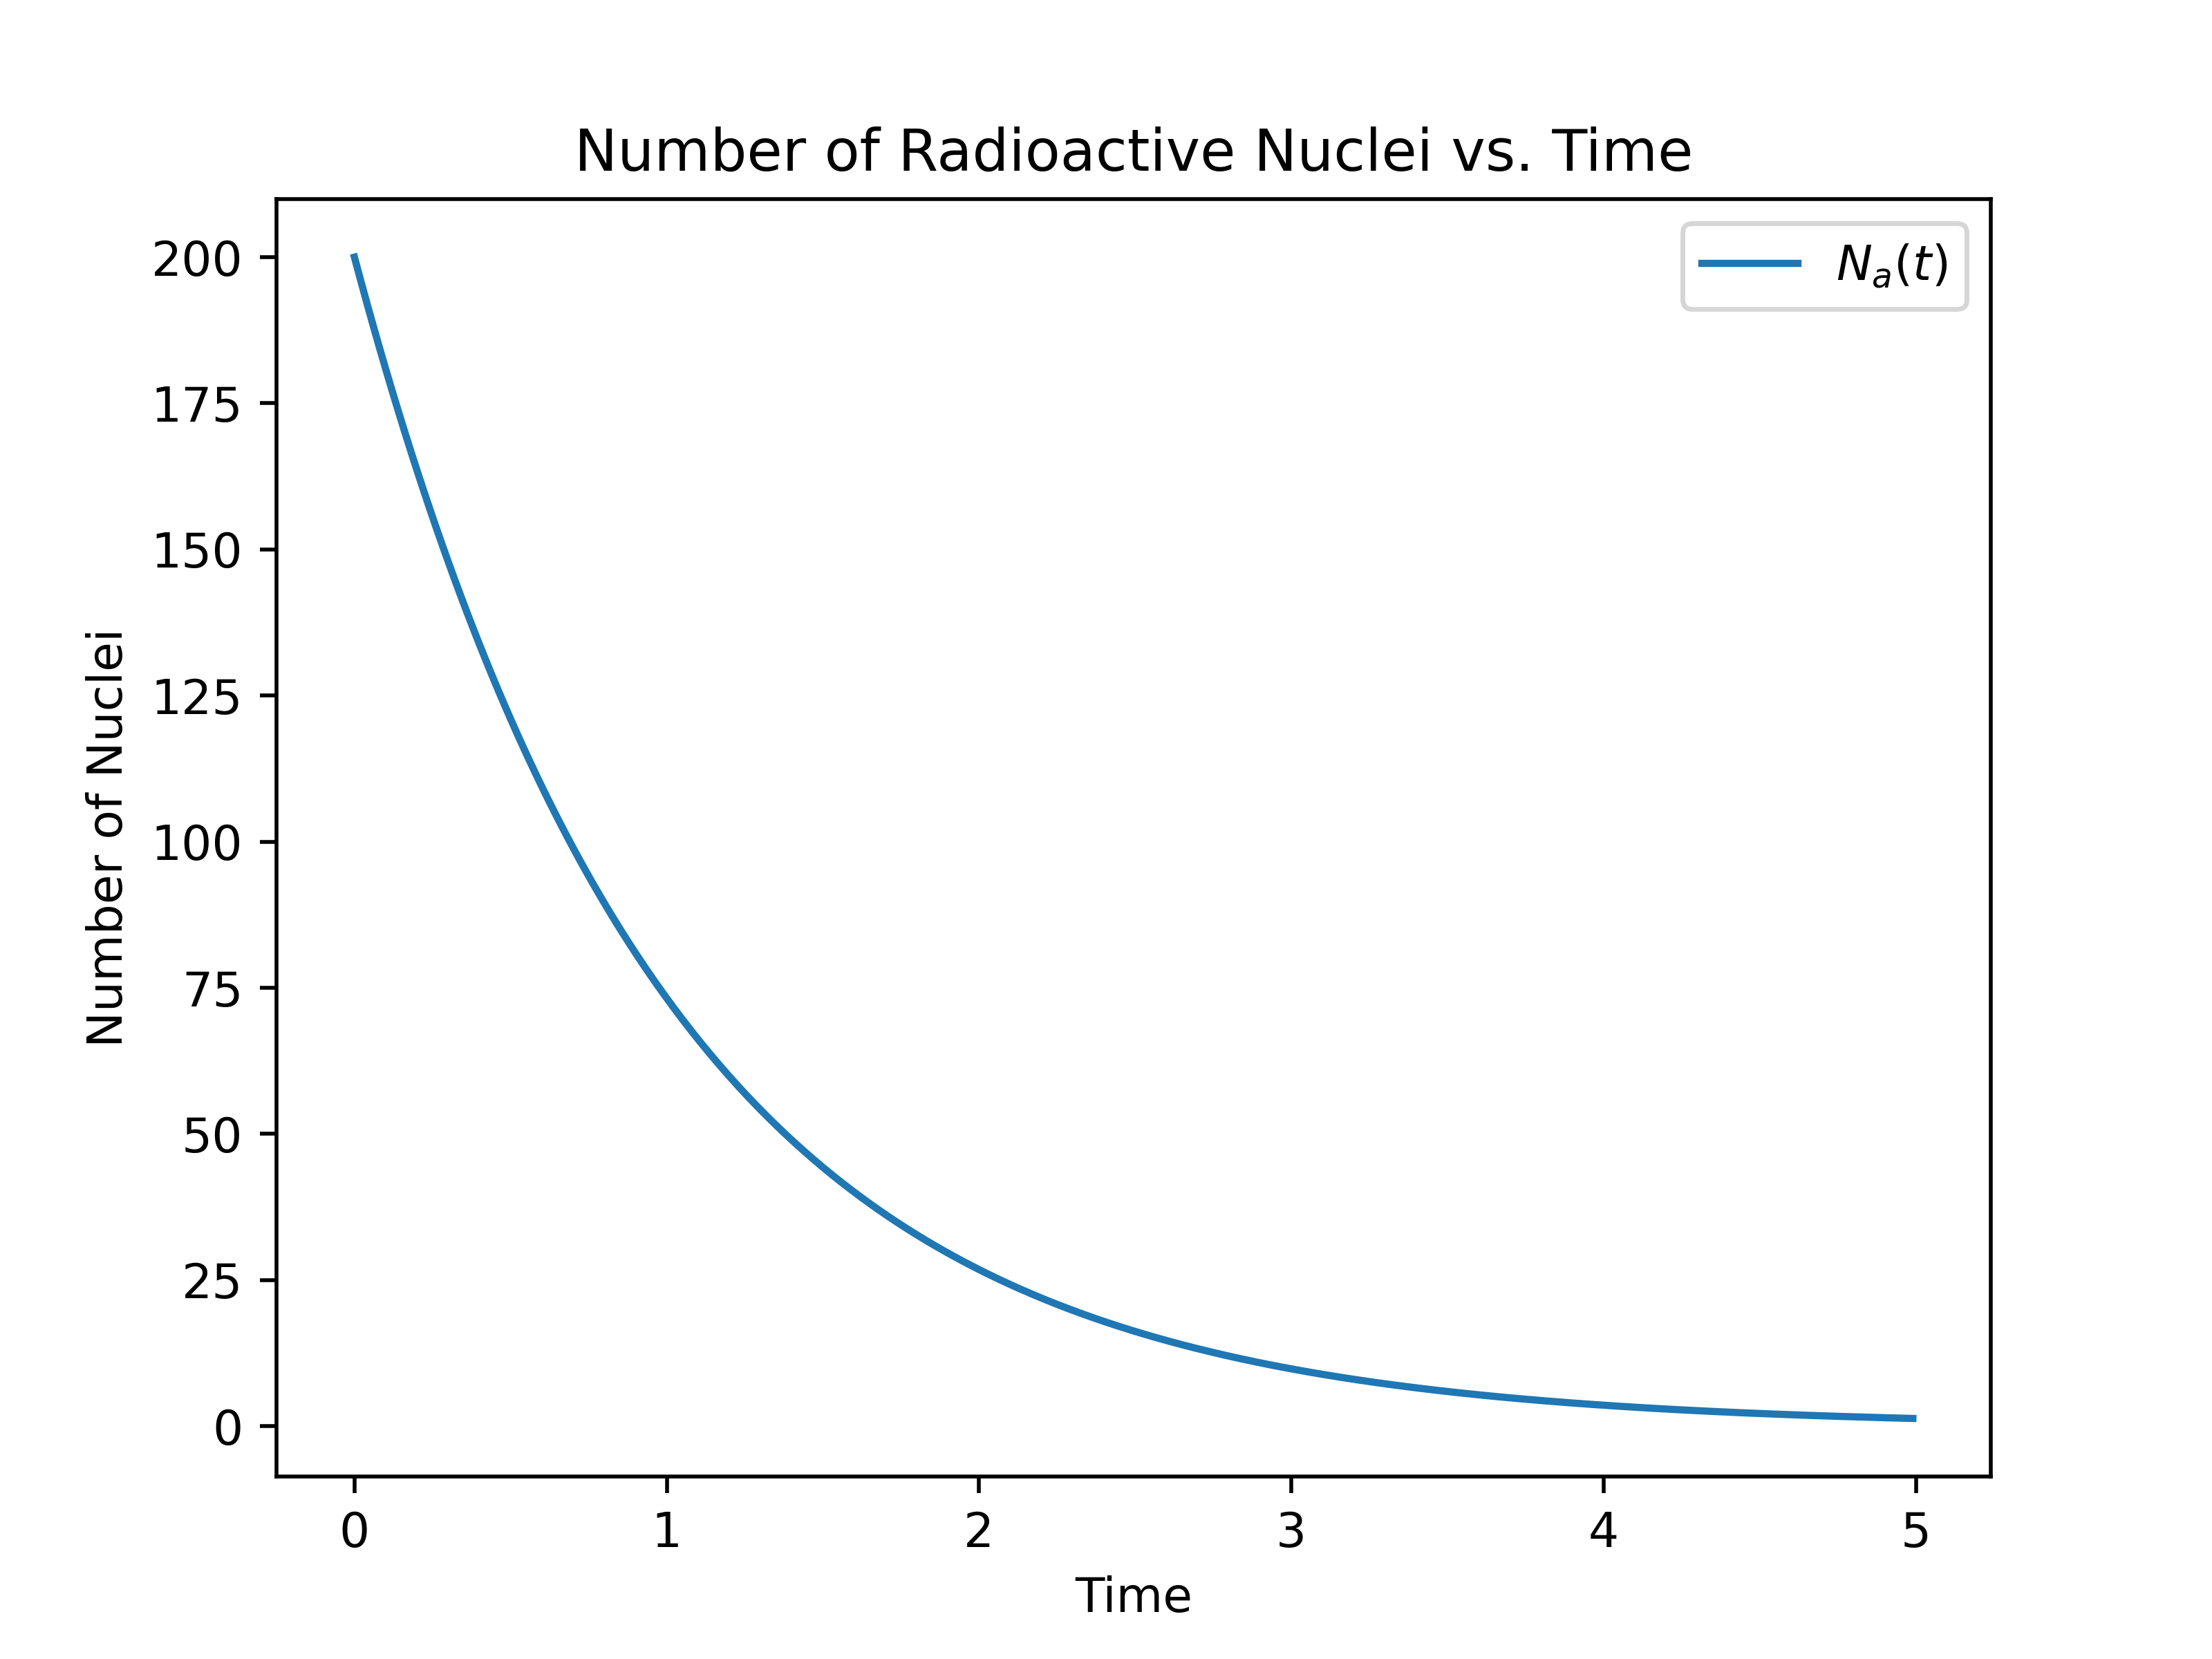
\includegraphics[scale=0.50]{Nuclei_A_0.01.png}
\caption{The decay of nuclei particles A over time.}\label{Proj1LessThan}
\end{figure}

The decay of nuclei A reflects a standard decay model. There is an exponential decline in the number of A particles which, given infinite time, would reach its limit of 0. Since the decay of nuclei A is not dependent upon nuclei B, we can compare this outcome to each of the different scenarios. 

\par We will then compare the decay of nuclei A and the decay of nuclei B where \(\tau_A > \tau_B\) and \(\tau_b = 0.5\):

\begin{figure}[H]
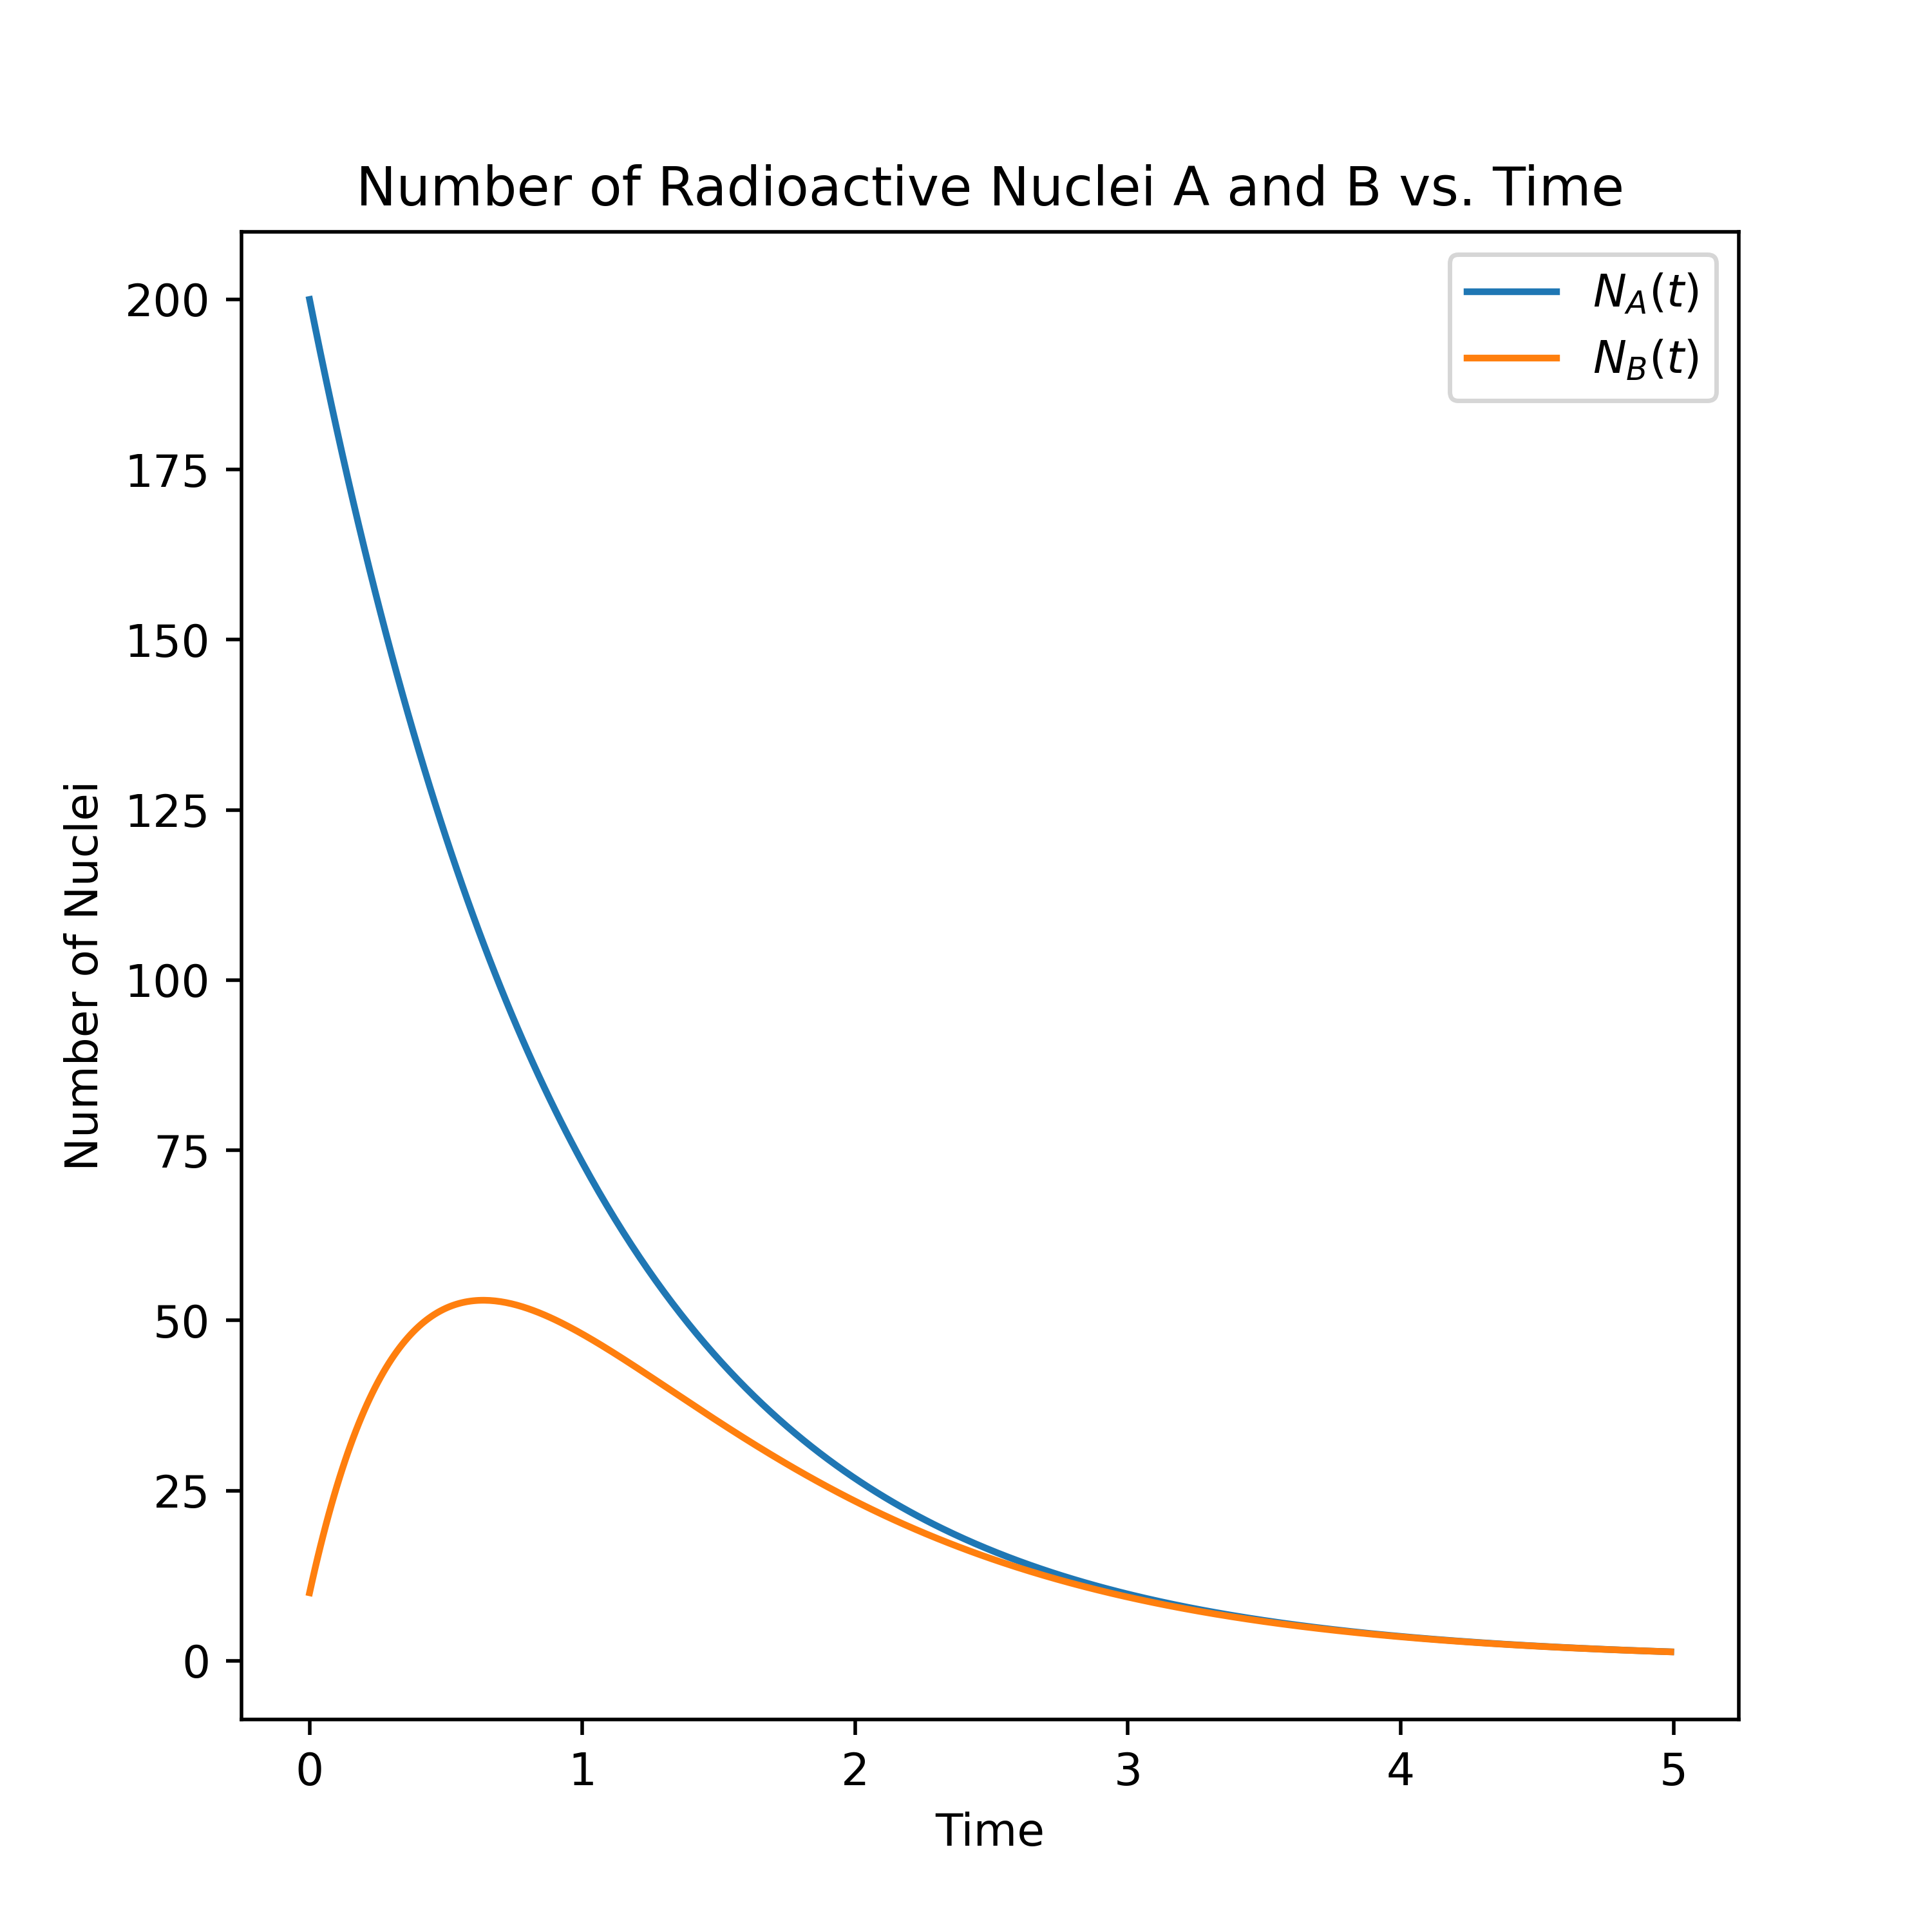
\includegraphics[scale=0.50]{Nuclei_AB_0.5_0.01.png}
\caption{The decay of nuclei particles A and B over time where \(\tau_A > \tau_B\) and \(\tau_B = 0.5\).}
\end{figure}

As we see in the figure 2 above, the decay of nuclei B peaks and then fades off as less of the nuclei A decay into nuclei B. While the graph for nuclei A shows a standard decay model, the graph for nuclei B reflects the changes as more and more of nuclei A decay over time. There is a point in which both have the same value as they both decay off towards 0.

\par Next, we will look at the situation where \(\tau_A = \tau_B = 1\):

\begin{figure}[H]
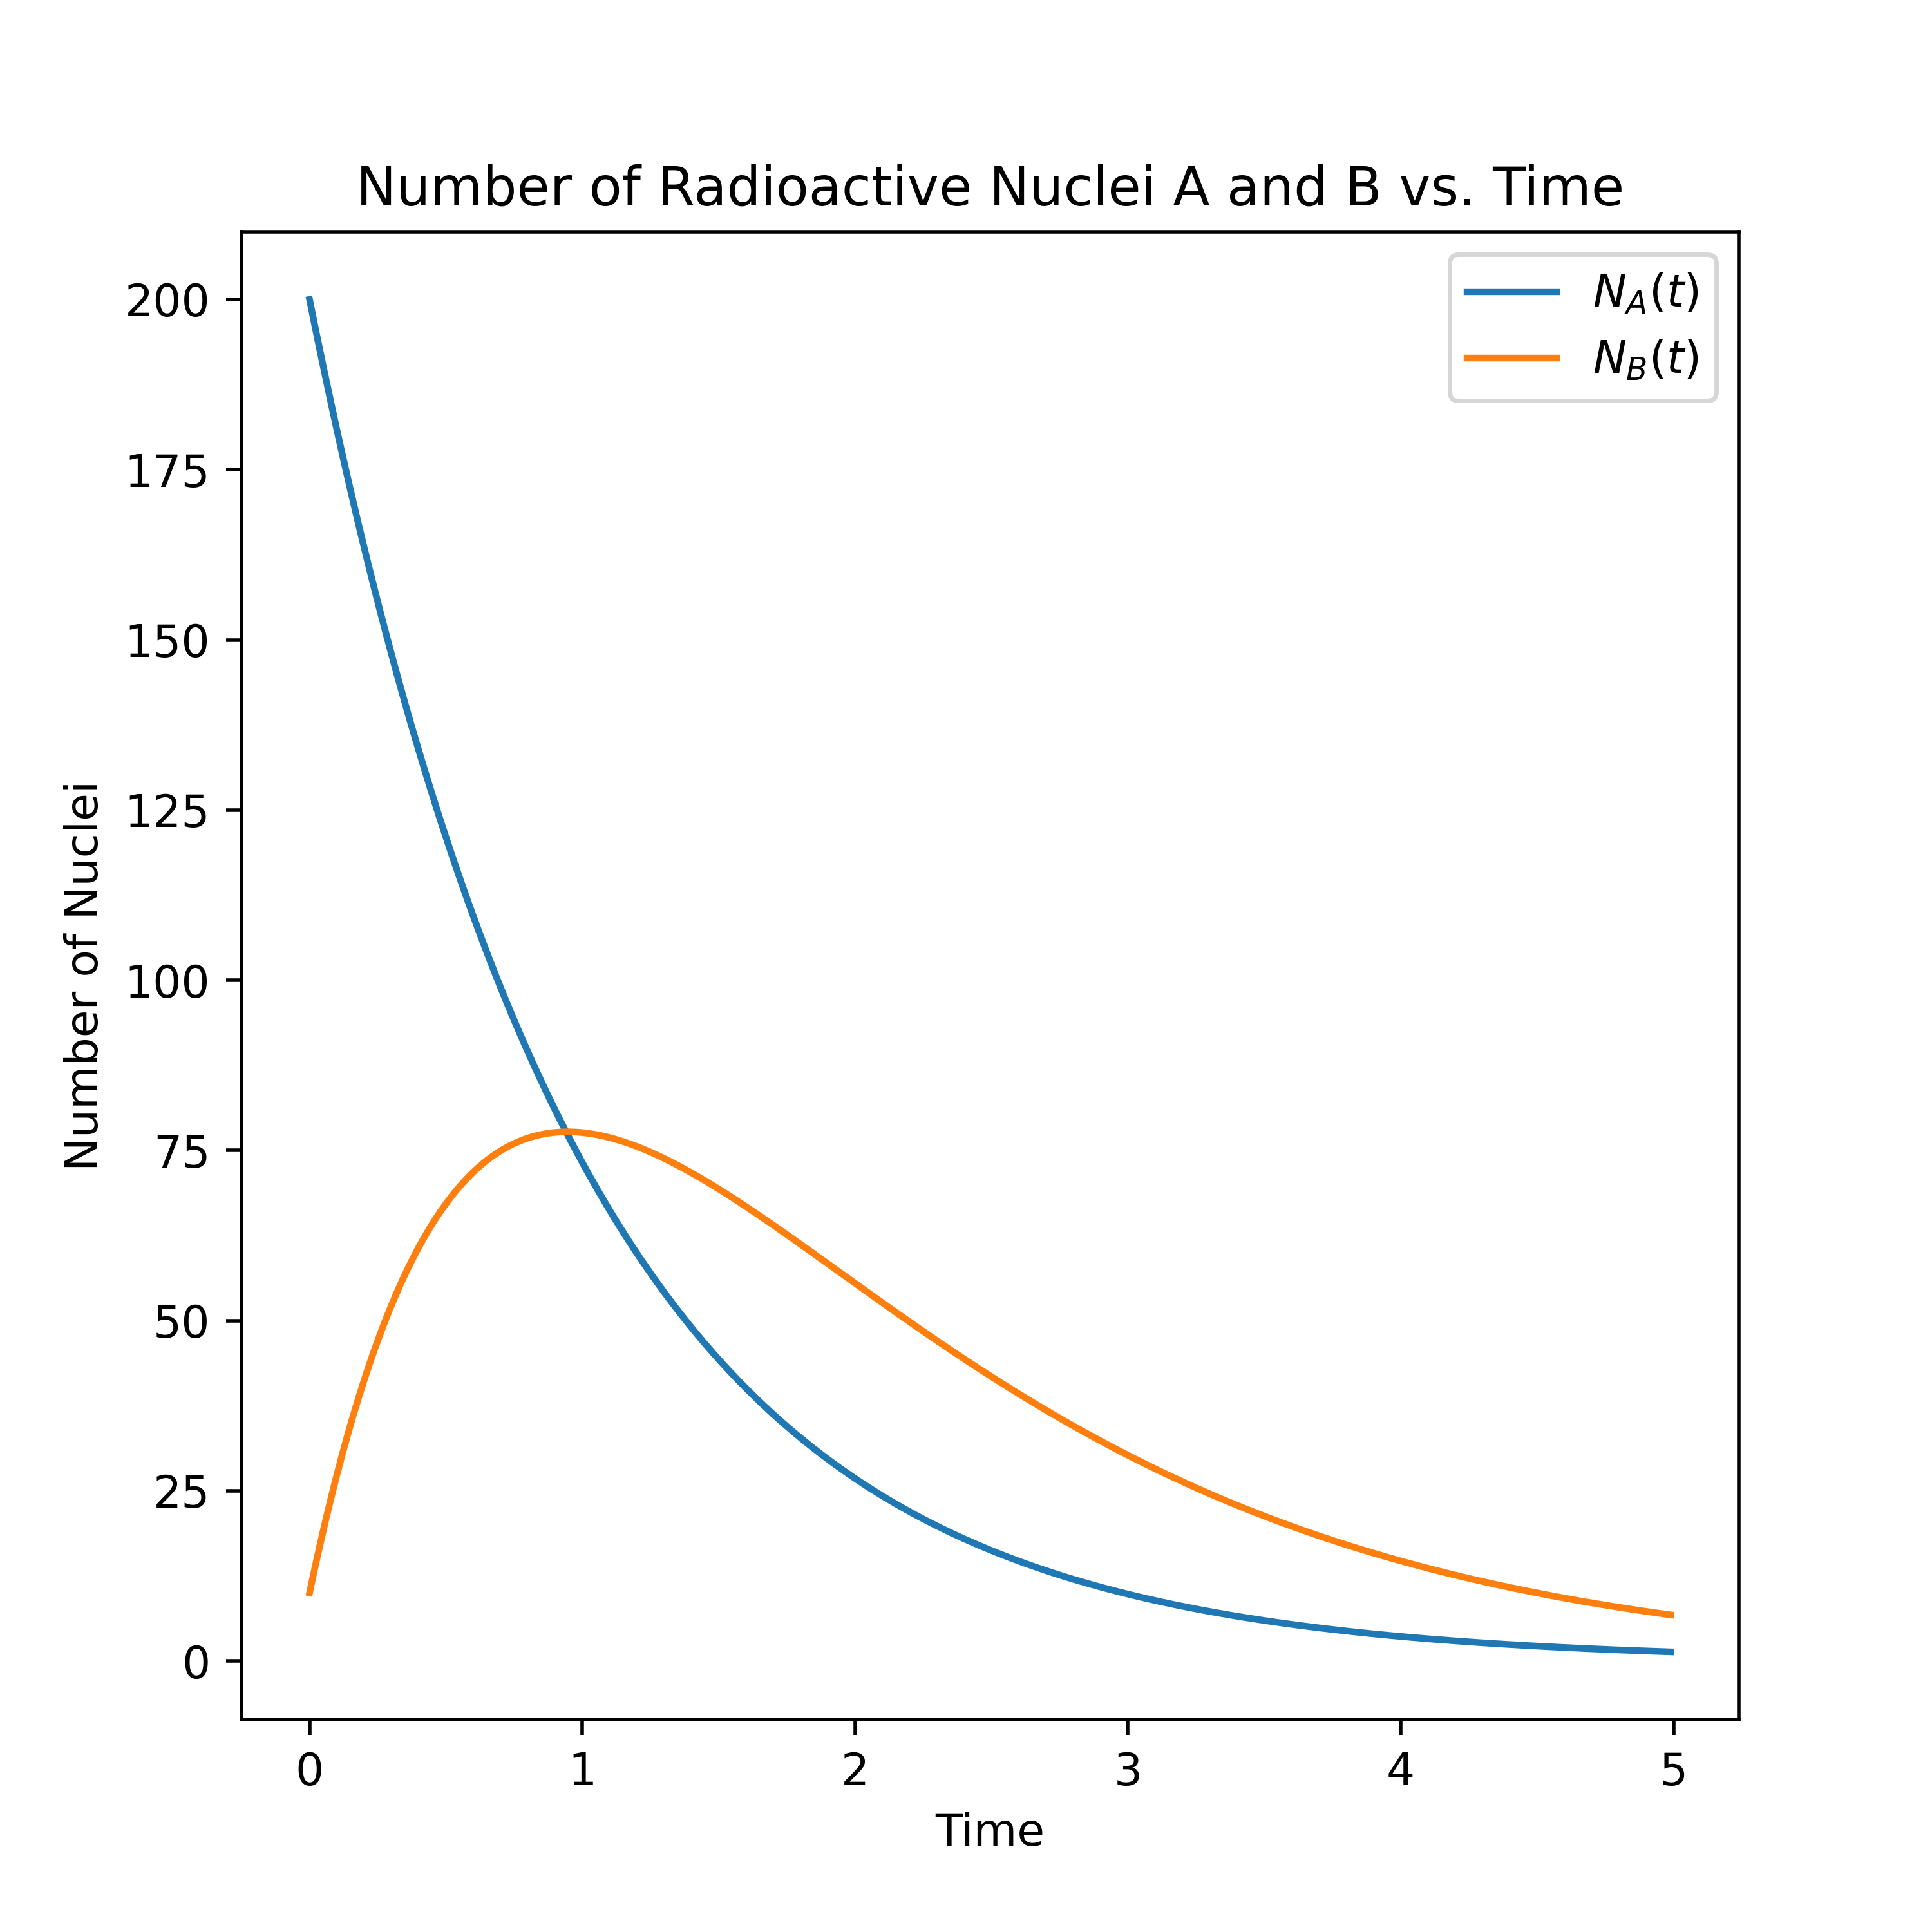
\includegraphics[scale=0.50]{Nuclei_AB_1_0.01.png}
\caption{The decay of nuclei particles A and B over time where \(\tau_A = \tau_B = 1\).}
\end{figure}

As we see here, the decay of nuclei B again shows a spike up to a peak and then a steady decline as of nuclei A decay into nuclei B. As compared to the situation where \(\tau_B = 0.5\), the peak is greater but the drop off is more gradual. Since it takes more time for nuclei B to decay, there are more of the original nuclei B as nuclei A decays into B.

\par Finally, we will look at the situation where \(\tau_A < \tau_B\) and \(\tau_B = 1.5\):

\begin{figure}[H]
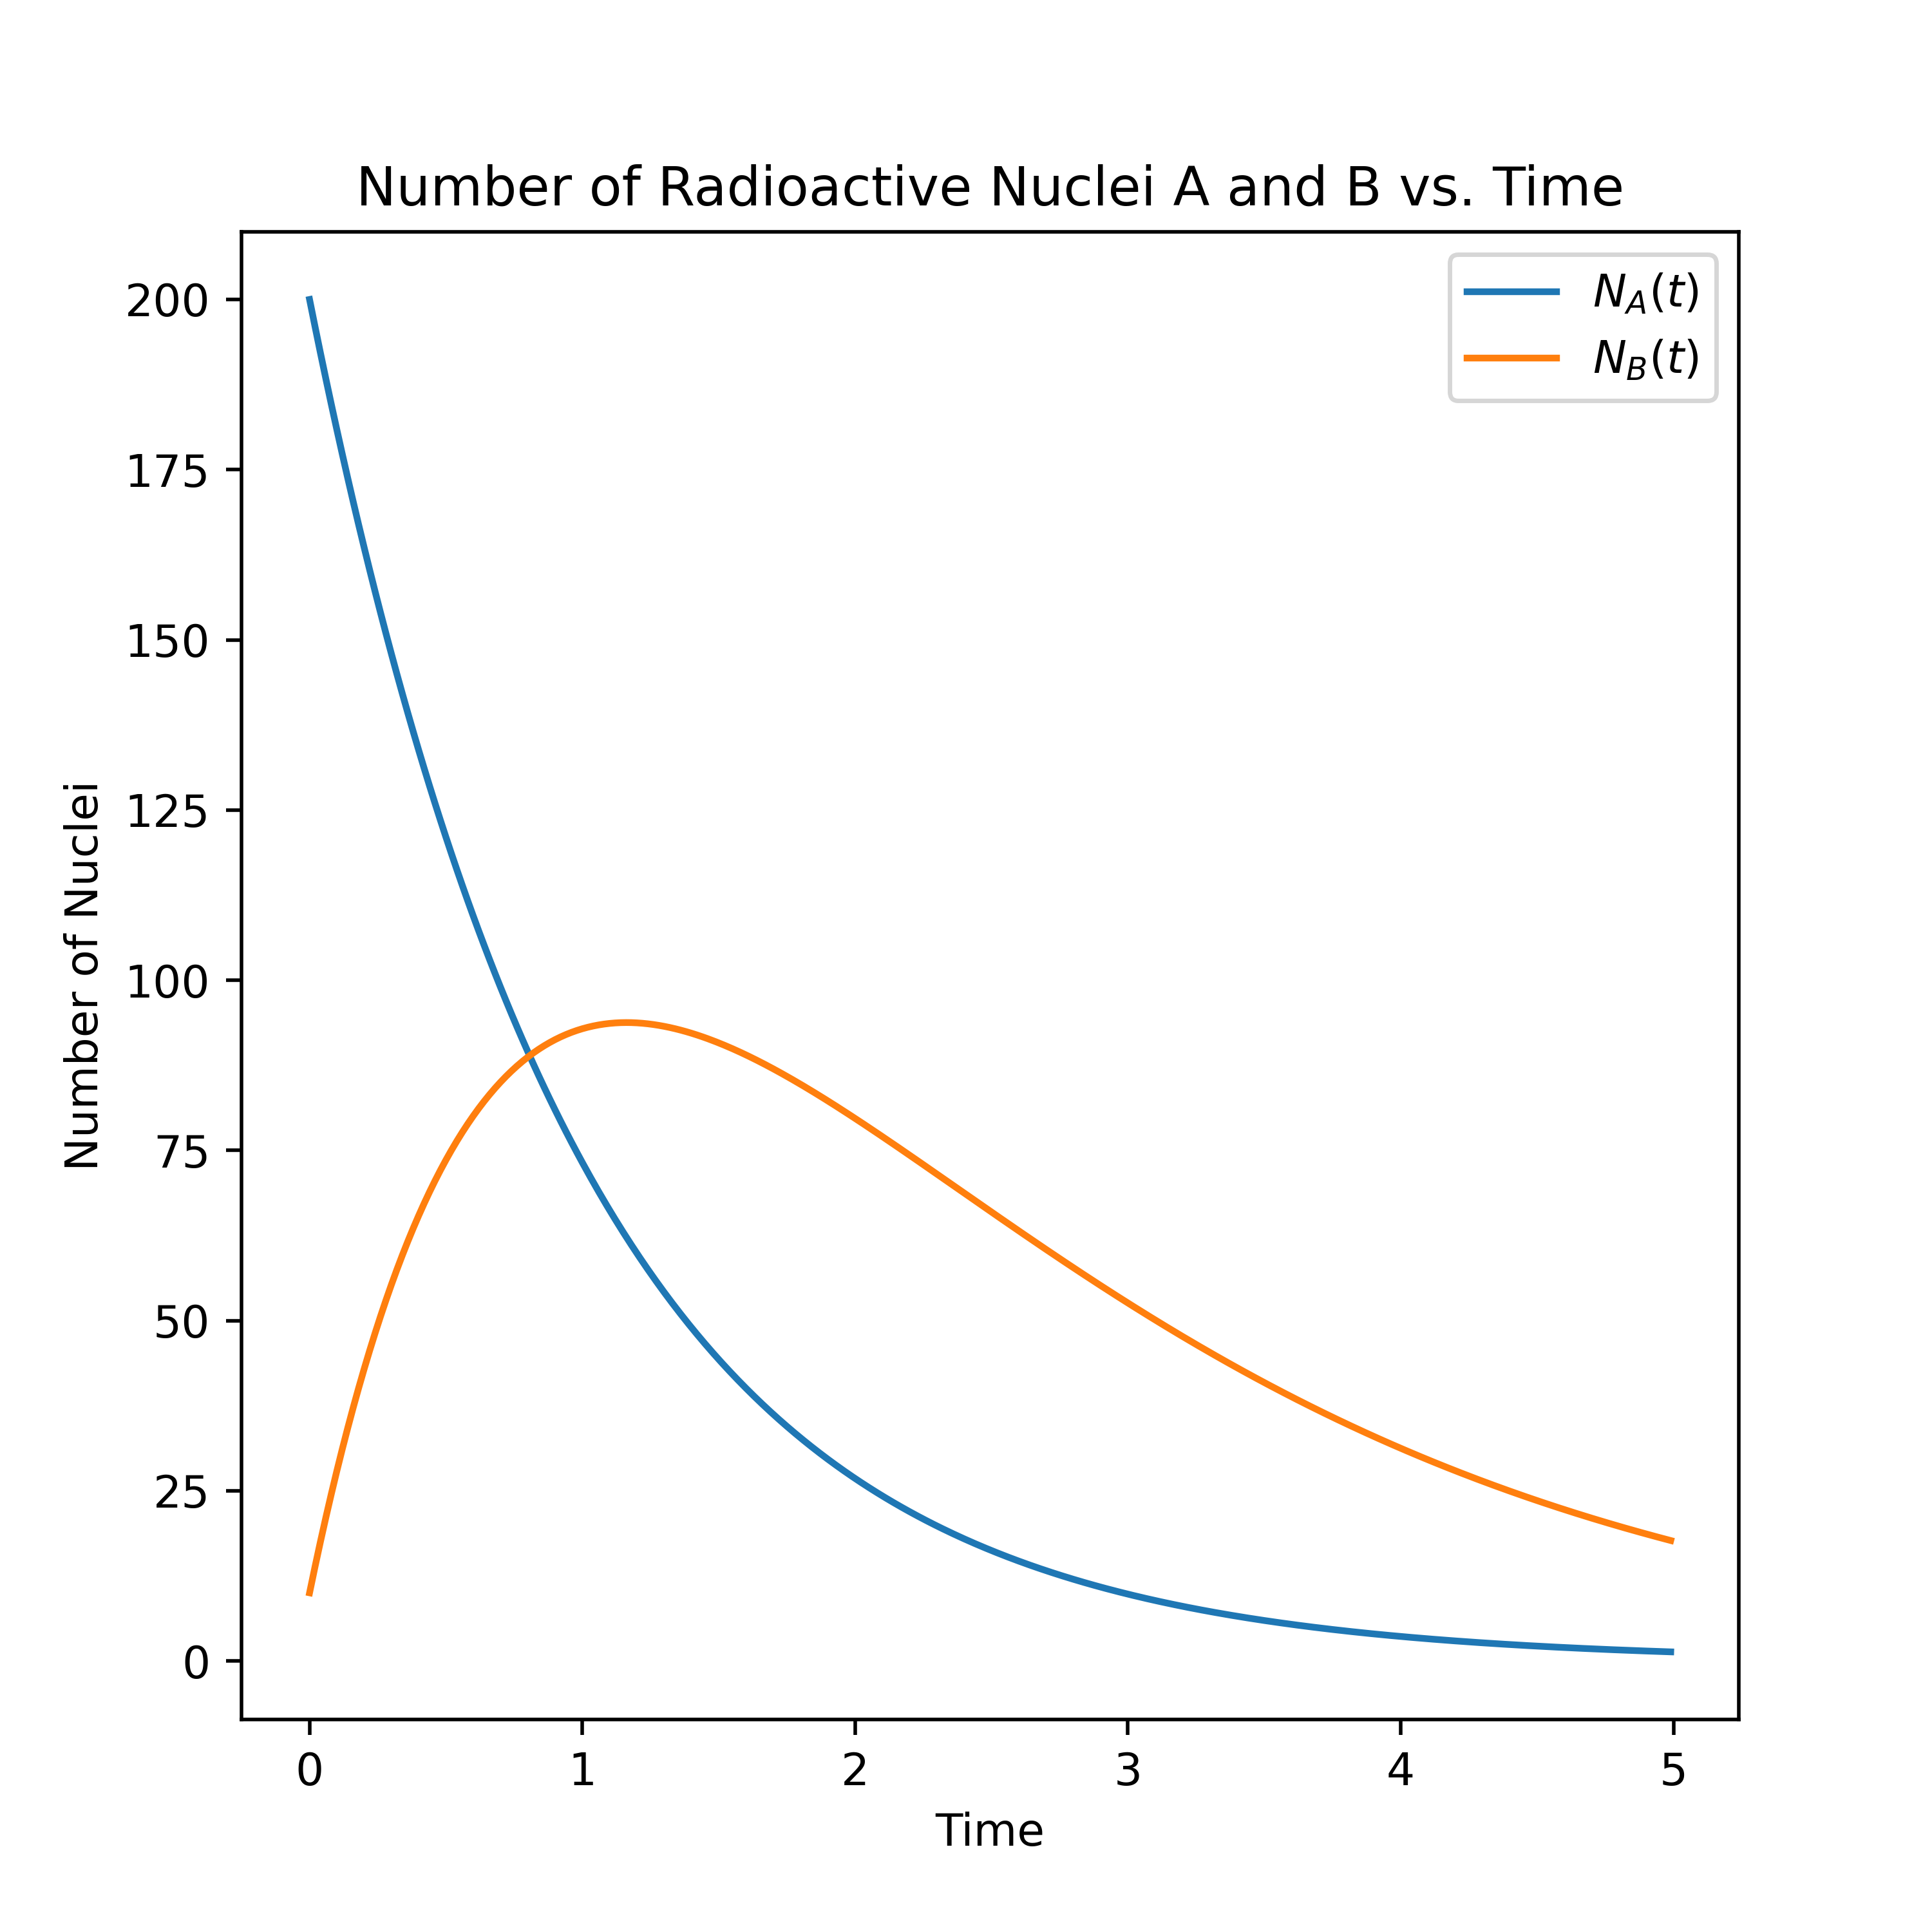
\includegraphics[scale=0.50]{Nuclei_AB_1.5_0.01.png}
\caption{The decay of nuclei particles A and B over time where \(\tau_A < \tau_B\) and \(\tau_B = 1\).}\label{Proj1Equal}
\end{figure}

In the final situation, in figure 4 we see that nuclei B decays at a slower rate. Since the decay constant is greater, we also see that the number of nuclei B peaks at a greater number and trails off at a slower rate as we saw with the situation with the equal decay constants. This is due to the fact that it takes more time for nuclei B to decay.

\par Comparing the different situations shows that the time constant plays an important part in how the system evolves over time. Going from Figure 2 to Figure 3, we see that the system decays at a slower rate due to the larger time constant. The system also peaks later and has a larger amplitude. This is reflective of the fact that there are more of the original nuclei B particles than with a lower time constant. This is further reinforced by looking at Figure 4 which draws out further and has an even greater peak.

\par We can see this more clearly by looking at each of the equations for nuclei B side by side.

\begin{figure}[H]
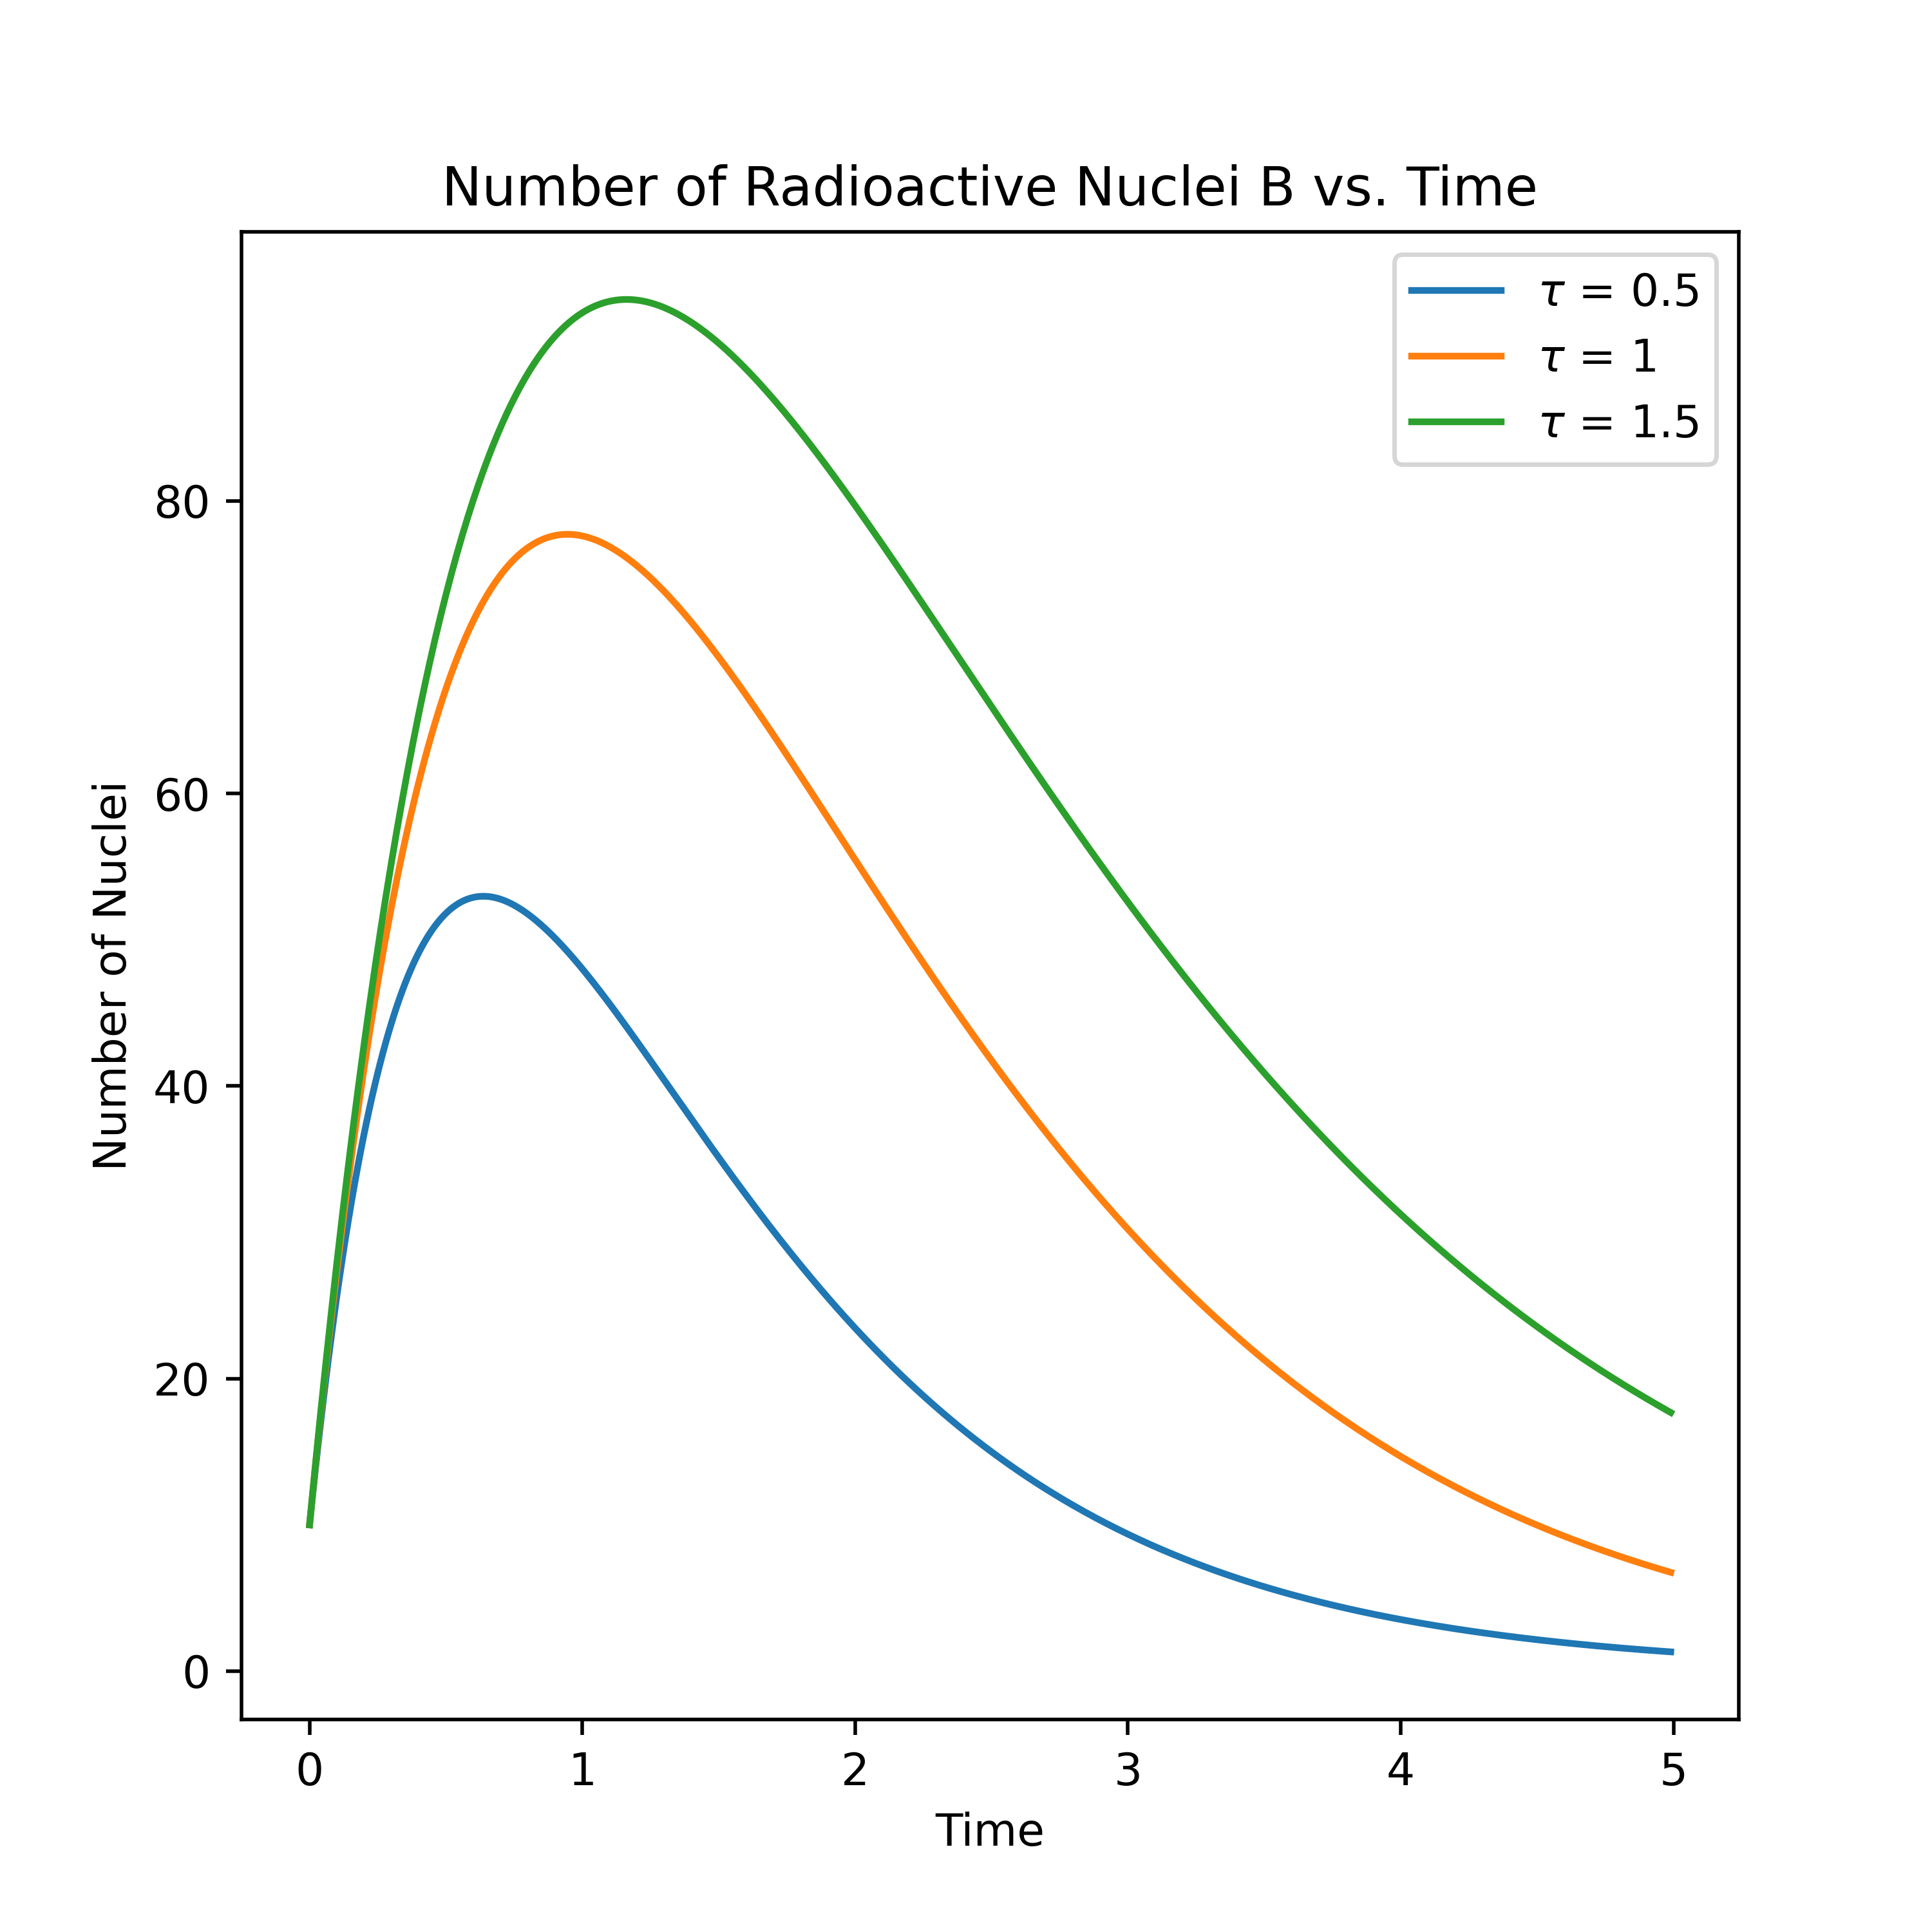
\includegraphics[scale=0.50]{Nuclei_B_0.01.png}
\caption{The comparison of the decay of nuclei A between the numeric approach and the analytical approach.}
\end{figure}

Figure 5 shows our conclusions clearly. As the time scale goes up, the maximum value goes up and occurs at a later time.

\par For the final part of my analysis, we explore the effectiveness of our methodology. Since the Euler method for approximation was used in each of the graphs, it is important to explore just how accurate of an approximation it really is. As such, here is the comparison of the nuclei A numeric approximation in Equation 8 with analytical solution in Equation 10:

\begin{figure}[H]
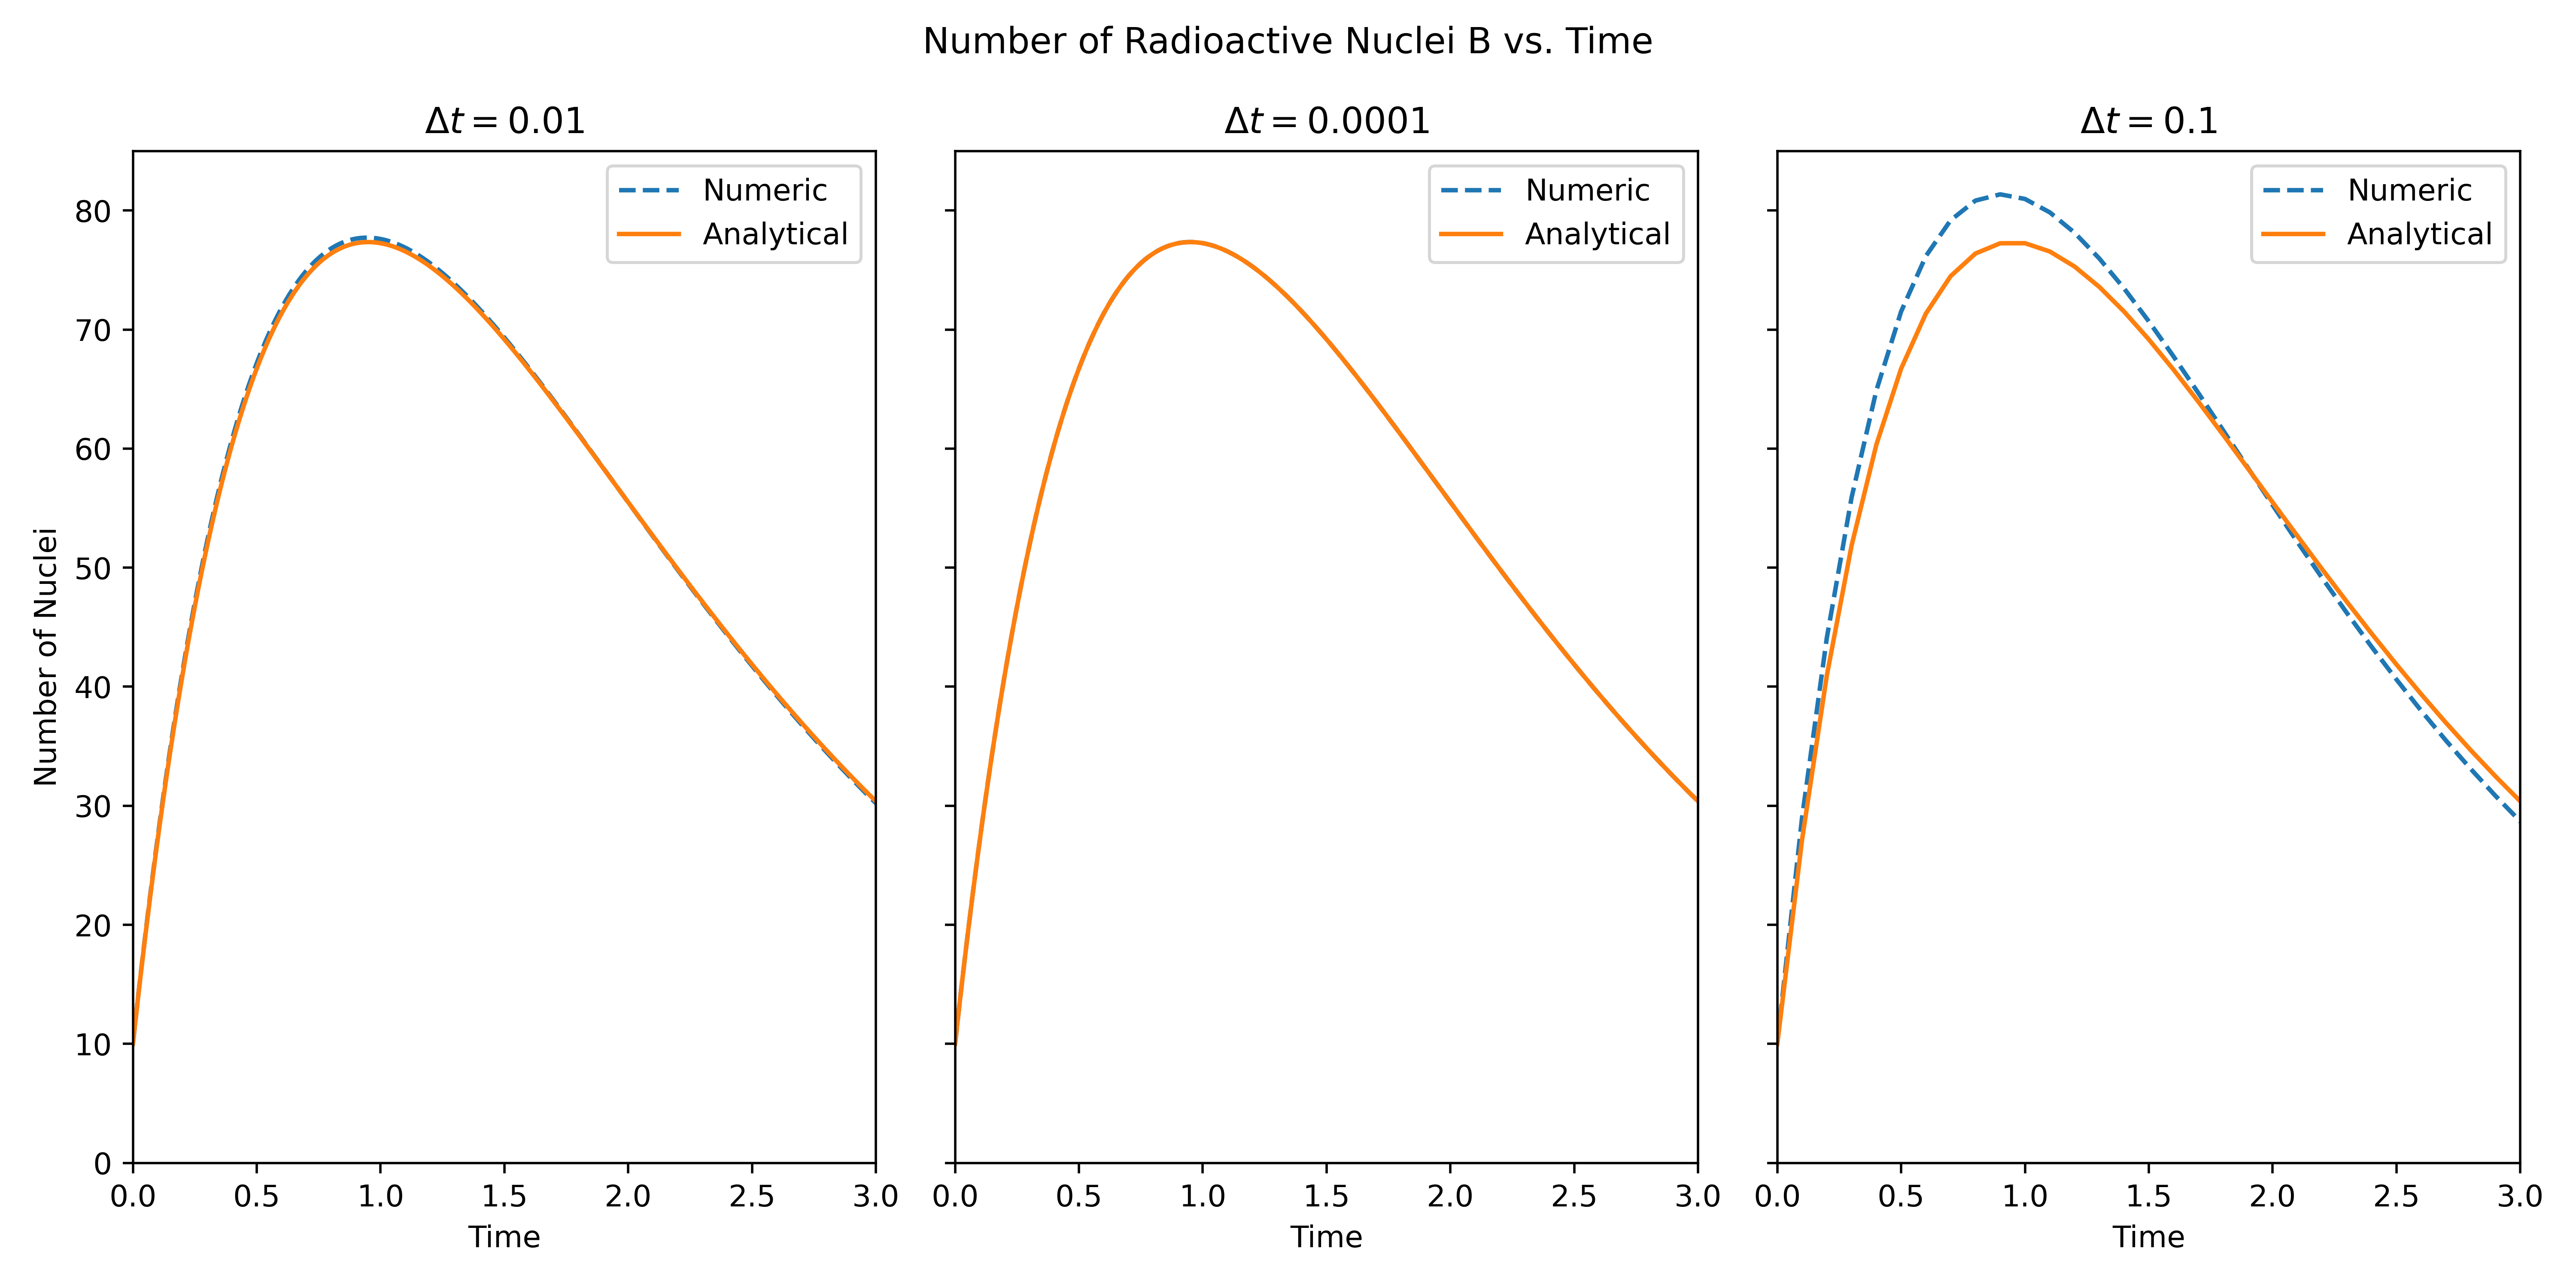
\includegraphics[scale=0.28]{Nuclei_AB_comp.png}
\caption{The comparison of the Euler approximation at different time steps to the analytical solution.}
\end{figure}

In figure 6, we see that the time step has an impact on how close the approximation is to the analytical solution. The time step used for our approximation earlier, $\Delta t = 0.01$, does have a small deviation from the analytical solution, especially when looking at the maximum. As we go from 0.01 to 0.0001, we can see that the numeric solution is almost identical to the analytical one. Finally, with a time step of 0.1, we can see that there is a large deviation from the analytical solution that makes if almost impractical to use.



\section{Conclusion} 
\label{sec:conclusion}


As shown in the graphs above, manipulating the time constant for nuclei B had no effect on the number of radioactive nuclei for A. However, the effect on B was quite significant. Modifying the time constant for nuclei B shows the impact it has on the evolving system.

\par As the time constant increased, the number of particles at any given time also increased. This is reflected in the differences in the peaks of the graphs. This would be represented in the real world as the number of the original particles of nuclei B remaining while nuclei A decayed into nuclei B. Eventually the decay of B particles becomes greater than the decay of A particles and thus it falls off. In addition, the use of the Euler approximation for the equations was sufficient to represent the analytical solution, as shown above..

\begin{thebibliography}{9}
\bibitem{Giordano6}
Nicholas J. Giordano and Hisao Nakanish,
\textit{Computational Physics}, 
(Pearson Prentice Hall, New Jersey,
Second Edition,
2005).
\end{thebibliography}

\end{document}